\documentclass[10pt]{ctexart}
\usepackage{mypackages}
%\usepackage[UTF8]{ctex} 

\renewcommand{\contentsname}{\erhao\song{\textbf{目\quad 录}}}
\setcounter{tocdepth}{2}
%\titlecontents{chapter}[0em]{\vspace{3pt}\xiaosi\song\bf}%
%{\prechaptername\CJKnumber{\thecontentslabel}\postchaptername\quad}{} %
%{\hspace{.5em}\titlerule*[7pt]{.}\xiaosi\contentspage}
%\titlecontents{section}[2em]{\vspace{3pt}\xiaosi\song} %
%{\thecontentslabel\quad}{} %
%{\hspace{.5em}\titlerule*[7pt]{.}\xiaosi\contentspage}
%\titlecontents{subsection}[4em]{\vspace{3pt}\xiaosi\song} %
%{\thecontentslabel\quad}{} %
%{\hspace{.5em}\titlerule*[7pt]{.}\xiaosi\contentspage}
%\renewcommand{\bibname}{参考文献}


\begin{document}
\begin{titlepage}
	\vspace*{-2cm}
	\flushleft
	% 
\includegraphics[width=0.7\textwidth]{figs/CUGB_fig}\\
	\vspace{3.5cm}
	\begin{center}
		\textbf{\song\yihao 《现代图论》\\[15pt] 大作业课题报告}
	\end{center}
	\vspace{3cm}
	\begin{center}
		\erhao \stxihei \parbox[t]{10em}
		{ \textbf{这里是你的题目} }
	\end{center}
	\vspace{2cm}
	\begin{center}
		\song\zihao{-3}
		\renewcommand\arraystretch{1.5}
		\begin{tabular}{p{2.5cm}c}
			\makebox[6em][s]{学生姓名:}  & \underline{\makebox[15em][c]{X}}      \\
			\makebox[6em][s]{学科、专业:} & \underline{\makebox[15em][c]{应用数学}}   \\
			\makebox[6em][s]{学号:}    & \underline{\makebox[15em][c]{x}}      \\
			\makebox[6em][s]{完成日期:}  & \underline{\makebox[15em][c]{\today}} \\
		\end{tabular}
		
		\vspace{3cm}
		{\hwxk \xiaoerhao 大连理工大学}
		
		\vspace*{5pt}
		{\zihao{-4} Dalian University of Technology}
	\end{center}
\end{titlepage}





\xiaosihao
\tableofcontents%设置目录
\thispagestyle{empty}
\clearpage
\bibliographystyle{unsrt}
\setcounter{page}{1}


\newpage


\textbf{\heiti 摘要:} 本文从。


\textbf{\heiti 关键词:} 时

\section{引言}


% TODO: \usepackage{graphicx} required
\begin{figure}[H]
	\centering
	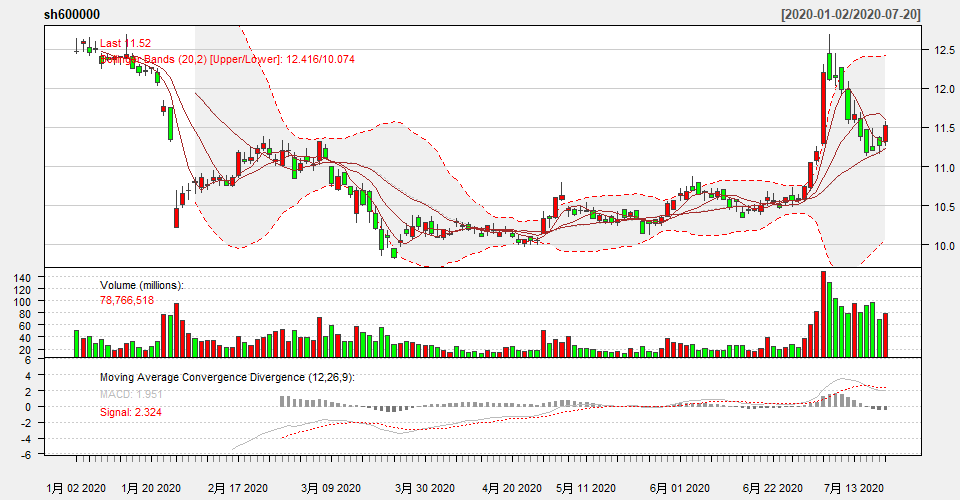
\includegraphics[width=0.95\linewidth]{figs/1}
	\caption[图1]{浦发银行(sh600000)2020年K线图及指标图}
	\label{fig:1}
\end{figure}






\section{指标选择及描述}
由于在此也不作进一步分析。

\section{模型建立}

\subsection{时序数据平滑化}

处


虽然从图上看,随着$k$的增大,图像变得越来越平滑,但也因此失去了一部分的信息,所以此时选取$k=7$进行平滑处理即可。

\subsection{指数预测模型}

指、


\subsection{ARIMA模型}

ARIMA模溯的观测值的数量。


\section{模型求解}

根据上面的模型建立过程,直接调用R中的函数求解如下:

\subsection{指数模型}

使用forecast包中的forecast()函数进行预测,可得到



上述结果中,浅灰和深灰的部分分别代表预测结果的80\%和95\%置信区间。

\subsection{ARIMA模型}




\section{结果分析}

断。


\section{总结与体会}

\subsection{论文总结}

本文

\subsection{心得体会}

在高。


\begin{thebibliography}{1}
	
	\bibitem{1}
	R.~I.Kabacoff.
	\newblock {\em R语言实战(第2版)}.
	\newblock 人民邮电出版社, 2016.
	
	
	\bibitem{2}
	范剑青, 姚琦伟著, 陈敏译.
	\newblock {\em 非线性时间序列—建模、预报及应用}.
	\newblock  北京:高等教育出版社, 2005.
	
	
	\bibitem{3}
	陈小玲.
	\newblock {\em 基于ARIMA模型与神经网络模型的股价预测}.
	\newblock 经济数学, 2017, 34(4).
	
\end{thebibliography}


\section{附录}

\subsection{源代码}

i


\subsection{数据包}

日线




\end{document}
